\documentclass[tikz,border=10pt]{standalone}
\usepackage{tikz}
\usepackage{xcolor}
\usetikzlibrary{shapes,arrows,positioning,calc}

\definecolor{solvercolor}{RGB}{209,196,233}
\definecolor{integratorcolor}{RGB}{200,230,201}
\definecolor{pinncolor}{RGB}{255,249,196}
\definecolor{datacolor}{RGB}{225,245,255}

\begin{document}
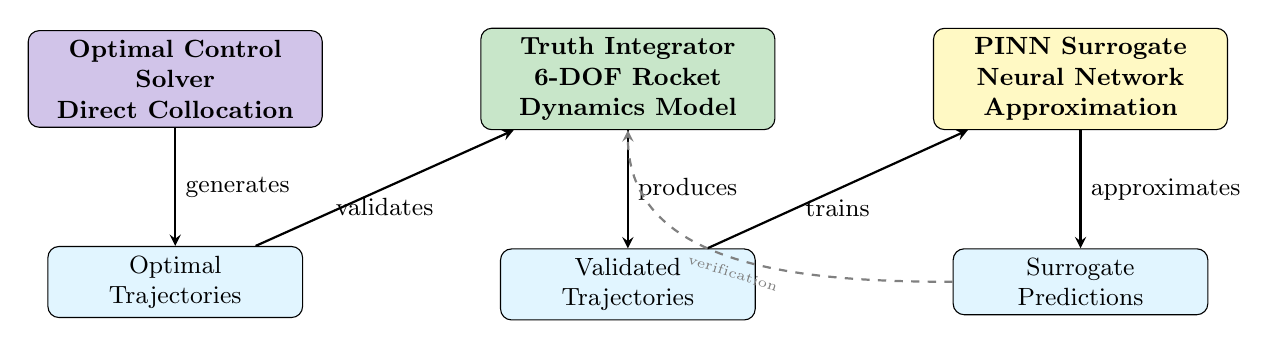
\begin{tikzpicture}[
    node distance=1.5cm and 2cm,
    every node/.style={font=\small},
    solver/.style={rectangle, rounded corners, fill=solvercolor, draw=black, text width=3.5cm, text centered, minimum height=1.2cm, font=\small\bfseries},
    integrator/.style={rectangle, rounded corners, fill=integratorcolor, draw=black, text width=3.5cm, text centered, minimum height=1.2cm, font=\small\bfseries},
    pinn/.style={rectangle, rounded corners, fill=pinncolor, draw=black, text width=3.5cm, text centered, minimum height=1.2cm, font=\small\bfseries},
    data/.style={rectangle, rounded corners, fill=datacolor, draw=black, text width=3cm, text centered, minimum height=0.8cm, font=\small},
    arrow/.style={->, >=stealth, thick, black},
    label/.style={font=\tiny, above, sloped}
]

% Main components - arranged horizontally
\node[solver] (solver) {Optimal Control\\Solver\\Direct Collocation};

\node[integrator, right=of solver] (integrator) {Truth Integrator\\6-DOF Rocket\\Dynamics Model};

\node[pinn, right=of integrator] (pinn) {PINN Surrogate\\Neural Network\\Approximation};

% Data flow - training dataset
\node[data, below=1.5cm of solver] (trajectories) {Optimal\\Trajectories};

\node[data, below=1.5cm of integrator] (validated) {Validated\\Trajectories};

\node[data, below=1.5cm of pinn] (predictions) {Surrogate\\Predictions};

% Arrows showing relationships
% Solver generates optimal trajectories
\draw[arrow] (solver) -- (trajectories) node[midway, right, font=\small] {generates};

% Trajectories validated by integrator
\draw[arrow] (trajectories) -- node[midway, below, font=\small] {validates} (integrator);

% Integrator produces validated trajectories
\draw[arrow] (integrator) -- (validated) node[midway, right, font=\small] {produces};

% Validated trajectories train PINN
\draw[arrow] (validated) -- node[midway, below, font=\small] {trains} (pinn);

% PINN makes predictions
\draw[arrow] (pinn) -- (predictions) node[midway, right, font=\small] {approximates};

% Feedback/verification arrow from PINN predictions back to integrator
\draw[arrow, dashed, gray] (predictions) to[out=180, in=270] node[midway, below, font=\tiny, sloped] {verification} (integrator);

\end{tikzpicture}
\end{document}

